\documentclass[journal,12pt,twocolumn]{IEEEtran}
%
\usepackage{setspace}
\usepackage{gensymb}
%\doublespacing
\singlespacing

%\usepackage{graphicx}
%\usepackage{amssymb}
%\usepackage{relsize}
\usepackage[cmex10]{amsmath}
%\usepackage{amsthm}
%\interdisplaylinepenalty=2500
%\savesymbol{iint}
%\usepackage{txfonts}
%\restoresymbol{TXF}{iint}
%\usepackage{wasysym}
\usepackage{amsthm}
%\usepackage{iithtlc}
\usepackage{mathrsfs}
\usepackage{txfonts}
\usepackage{stfloats}
\usepackage{bm}
\usepackage{cite}
\usepackage{cases}
\usepackage{subfig}
%\usepackage{xtab}
\usepackage{longtable}
\usepackage{multirow}
%\usepackage{algorithm}
%\usepackage{algpseudocode}
\usepackage{enumitem}
\usepackage{mathtools}
\usepackage{steinmetz}
\usepackage{tikz}
\usepackage{circuitikz}
\usepackage{verbatim}
\usepackage{tfrupee}
\usepackage[breaklinks=true]{hyperref}
%\usepackage{stmaryrd}
\usepackage{tkz-euclide} % loads  TikZ and tkz-base
\usetkzobj{all}
\usetikzlibrary{decorations.markings}
\usetikzlibrary{shapes.geometric}
\newif\iflabrev
\usepackage{listings}
    \usepackage{color}                                            %%
    \usepackage{array}                                            %%
    \usepackage{longtable}                                        %%
    \usepackage{calc}                                             %%
    \usepackage{multirow}                                         %%
    \usepackage{hhline}                                           %%
    \usepackage{ifthen}                                           %%
  %optionally (for landscape tables embedded in another document): %%
    \usepackage{lscape}     
\usepackage{multicol}
\usepackage{chngcntr}
%\usepackage{enumerate}

%\usepackage{wasysym}
%\newcounter{MYtempeqncnt}
\DeclareMathOperator*{\Res}{Res}
%\renewcommand{\baselinestretch}{2}
\renewcommand\thesection{\arabic{section}}
\renewcommand\thesubsection{\thesection.\arabic{subsection}}
\renewcommand\thesubsubsection{\thesubsection.\arabic{subsubsection}}

\renewcommand\thesectiondis{\arabic{section}}
\renewcommand\thesubsectiondis{\thesectiondis.\arabic{subsection}}
\renewcommand\thesubsubsectiondis{\thesubsectiondis.\arabic{subsubsection}}

% correct bad hyphenation here
\hyphenation{op-tical net-works semi-conduc-tor}
\def\inputGnumericTable{}                                 %%

\lstset{
%language=C,
frame=single, 
breaklines=true,
columns=fullflexible
}
%\lstset{
%language=tex,
%frame=single, 
%breaklines=true
%}

\begin{document}
%


\newtheorem{theorem}{Theorem}[section]
\newtheorem{problem}{Problem}
\newtheorem{proposition}{Proposition}[section]
\newtheorem{lemma}{Lemma}[section]
\newtheorem{corollary}[theorem]{Corollary}
\newtheorem{example}{Example}[section]
\newtheorem{definition}[problem]{Definition}
%\newtheorem{thm}{Theorem}[section] 
%\newtheorem{defn}[thm]{Definition}
%\newtheorem{algorithm}{Algorithm}[section]
%\newtheorem{cor}{Corollary}
\newcommand{\BEQA}{\begin{eqnarray}}
\newcommand{\EEQA}{\end{eqnarray}}
\newcommand{\define}{\stackrel{\triangle}{=}}
\bibliographystyle{IEEEtran}
%\bibliographystyle{ieeetr}
\providecommand{\mbf}{\mathbf}
\providecommand{\pr}[1]{\ensuremath{\Pr\left(#1\right)}}
\providecommand{\qfunc}[1]{\ensuremath{Q\left(#1\right)}}
\providecommand{\sbrak}[1]{\ensuremath{{}\left[#1\right]}}
\providecommand{\lsbrak}[1]{\ensuremath{{}\left[#1\right.}}
\providecommand{\rsbrak}[1]{\ensuremath{{}\left.#1\right]}}
\providecommand{\brak}[1]{\ensuremath{\left(#1\right)}}
\providecommand{\lbrak}[1]{\ensuremath{\left(#1\right.}}
\providecommand{\rbrak}[1]{\ensuremath{\left.#1\right)}}
\providecommand{\cbrak}[1]{\ensuremath{\left\{#1\right\}}}
\providecommand{\lcbrak}[1]{\ensuremath{\left\{#1\right.}}
\providecommand{\rcbrak}[1]{\ensuremath{\left.#1\right\}}}
\theoremstyle{remark}
\newtheorem{rem}{Remark}
\newcommand{\sgn}{\mathop{\mathrm{sgn}}}
\providecommand{\abs}[1]{\left\vert#1\right\vert}
\providecommand{\res}[1]{\Res\displaylimits_{#1}} 
\providecommand{\norm}[1]{\left\lVert#1\right\rVert}
%\providecommand{\norm}[1]{\lVert#1\rVert}
\providecommand{\mtx}[1]{\mathbf{#1}}
\providecommand{\mean}[1]{E\left[ #1 \right]}
\providecommand{\fourier}{\overset{\mathcal{F}}{ \rightleftharpoons}}
%\providecommand{\hilbert}{\overset{\mathcal{H}}{ \rightleftharpoons}}
\providecommand{\system}{\overset{\mathcal{H}}{ \longleftrightarrow}}
	%\newcommand{\solution}[2]{\textbf{Solution:}{#1}}
\newcommand{\solution}{\noindent \textbf{Solution: }}
\newcommand{\cosec}{\,\text{cosec}\,}
\providecommand{\dec}[2]{\ensuremath{\overset{#1}{\underset{#2}{\gtrless}}}}
\newcommand{\myvec}[1]{\ensuremath{\begin{pmatrix}#1\end{pmatrix}}}
\newcommand{\mydet}[1]{\ensuremath{\begin{vmatrix}#1\end{vmatrix}}}
%\numberwithin{equation}{section}
\numberwithin{equation}{subsection}
%\numberwithin{problem}{section}
%\numberwithin{definition}{section}
\makeatletter
\@addtoreset{figure}{problem}
\makeatother
\let\StandardTheFigure\thefigure
\let\vec\mathbf
%\renewcommand{\thefigure}{\theproblem.\arabic{figure}}
\renewcommand{\thefigure}{\theproblem}
%\setlist[enumerate,1]{before=\renewcommand\theequation{\theenumi.\arabic{equation}}
%\counterwithin{equation}{enumi}
%\renewcommand{\theequation}{\arabic{subsection}.\arabic{equation}}
\def\putbox#1#2#3{\makebox[0in][l]{\makebox[#1][l]{}\raisebox{\baselineskip}[0in][0in]{\raisebox{#2}[0in][0in]{#3}}}}
     \def\rightbox#1{\makebox[0in][r]{#1}}
     \def\centbox#1{\makebox[0in]{#1}}
     \def\topbox#1{\raisebox{-\baselineskip}[0in][0in]{#1}}
     \def\midbox#1{\raisebox{-0.5\baselineskip}[0in][0in]{#1}}
\vspace{3cm}
\title{
%	\logo{
Control Systems
%	}
}
\author{ G V V Sharma$^{*}$% <-this % stops a space
	\thanks{*The author is with the Department
		of Electrical Engineering, Indian Institute of Technology, Hyderabad
		502285 India e-mail:  gadepall@iith.ac.in. All content in this manual is released under GNU GPL.  Free and open source.}
	
}	
%\title{
%	\logo{Matrix Analysis through Octave}{\begin{center}\includegraphics[scale=.24]{tlc}\end{center}}{}{HAMDSP}
%}
% paper title
% can use linebreaks \\ within to get better formatting as desired
%\title{Matrix Analysis through Octave}
%
%
% author names and IEEE memberships
% note positions of commas and nonbreaking spaces ( ~ ) LaTeX will not break
% a structure at a ~ so this keeps an author's name from being broken across
% two lines.
% use \thanks{} to gain access to the first footnote area
% a separate \thanks must be used for each paragraph as LaTeX2e's \thanks
% was not built to handle multiple paragraphs
%
%\author{<-this % stops a space
%\thanks{}}
%}
% note the % following the last \IEEEmembership and also \thanks - 
% these prevent an unwanted space from occurring between the last author name
% and the end of the author line. i.e., if you had this:
% 
% \author{....lastname \thanks{...} \thanks{...} }
%                     ^------------^------------^----Do not want these spaces!
%
% a space would be appended to the last name and could cause every name on that
% line to be shifted left slightly. This is one of those "LaTeX things". For
% instance, "\textbf{A} \textbf{B}" will typeset as "A B" not "AB". To get
% "AB" then you have to do: "\textbf{A}\textbf{B}"
% \thanks is no different in this regard, so shield the last } of each \thanks
% that ends a line with a % and do not let a space in before the next \thanks.
% Spaces after \IEEEmembership other than the last one are OK (and needed) as
% you are supposed to have spaces between the names. For what it is worth,
% this is a minor point as most people would not even notice if the said evil
% space somehow managed to creep in.
% The paper headers
%\markboth{Journal of \LaTeX\ Class Files,~Vol.~6, No.~1, January~2007}%
%{Shell \MakeLowercase{\textit{et al.}}: Bare Demo of IEEEtran.cls for Journals}
% The only time the second header will appear is for the odd numbered pages
% after the title page when using the twoside option.
% 
% *** Note that you probably will NOT want to include the author's ***
% *** name in the headers of peer review papers.                   ***
% You can use \ifCLASSOPTIONpeerreview for conditional compilation here if
% you desire.
% If you want to put a publisher's ID mark on the page you can do it like
% this:
%\IEEEpubid{0000--0000/00\$00.00~\copyright~2007 IEEE}
% Remember, if you use this you must call \IEEEpubidadjcol in the second
% column for its text to clear the IEEEpubid mark.
% make the title area
\maketitle
\newpage
\tableofcontents
\bigskip
\renewcommand{\thefigure}{\theenumi}
\renewcommand{\thetable}{\theenumi}
%\renewcommand{\theequation}{\theenumi}
%\begin{abstract}
%%\boldmath
%In this letter, an algorithm for evaluating the exact analytical bit error rate  (BER)  for the piecewise linear (PL) combiner for  multiple relays is presented. Previous results were available only for upto three relays. The algorithm is unique in the sense that  the actual mathematical expressions, that are prohibitively large, need not be explicitly obtained. The diversity gain due to multiple relays is shown through plots of the analytical BER, well supported by simulations. 
%
%\end{abstract}
% IEEEtran.cls defaults to using nonbold math in the Abstract.
% This preserves the distinction between vectors and scalars. However,
% if the journal you are submitting to favors bold math in the abstract,
% then you can use LaTeX's standard command \boldmath at the very start
% of the abstract to achieve this. Many IEEE journals frown on math
% in the abstract anyway.
% Note that keywords are not normally used for peerreview papers.
%\begin{IEEEkeywords}
%Cooperative diversity, decode and forward, piecewise linear
%\end{IEEEkeywords}
% For peer review papers, you can put extra information on the cover
% page as needed:
% \ifCLASSOPTIONpeerreview
% \begin{center} \bfseries EDICS Category: 3-BBND \end{center}
% \fi
%
% For peerreview papers, this IEEEtran command inserts a page break and
% creates the second title. It will be ignored for other modes.
%\IEEEpeerreviewmaketitle
\begin{abstract}
This manual is an introduction to control systems based on GATE problems.Links to sample Python codes are available in the text.  
\end{abstract}
Download python codes using 
\begin{lstlisting}
svn co https://github.com/gadepall/school/trunk/control/codes
\end{lstlisting}
\section{Circuit Design}
%\begin{enumerate}[label=\arabic*.,ref=\theenumi]
\begin{enumerate}[label=\thesection.\arabic*.,ref=\thesection.\theenumi]
\numberwithin{equation}{enumi}
%2.1.1
\item Consider the Magnitude Bode Plot and Phase Bode Plot \ref{fig:ee18btech11014_Bode} of Open-Loop Transfer Function of an Amplifier. Estimate the Open-Loop Transfer Function. (Assume $'A'$ as $'G'$ and $'\beta'$ as $'H'$)
\begin{figure}[ht!]
	\begin{center}
		\includegraphics[width=\columnwidth]{./figs/ee18btech11014/ee18btech11014_figa.eps}
	\end{center}
	\caption{Magnitude and Phase Bode Plot}
	\label{fig:ee18btech11014_Bode}
\end{figure}
\\
\solution Let $G(f)$ be the Open-Loop Transfer Function,
\begin{align}
G(f) = 
\begin{cases} 
      100 & 0 < f < 10^{5} \\
      200-20\log(f) & 10^{5} < f < 10^{6} \\
      320-40\log(f) & 10^{6} < f < 10^{7} \\
      460-60\log(f) & 10^{7} < f  \\
\end{cases}
\end{align}

\begin{align}
\nabla G(f) &= \dfrac{d(G(f))}{d(\log(f))} =
\begin{cases} 
        0 & 0 < f < 10^{5} \\
      -20 & 10^{5} < f < 10^{6} \\
      -40 & 10^{6} < f < 10^{7} \\
      -60 & 10^{7} < f  \\ 
\end{cases}
\end{align}

As we know that, \textbf{When a pole is encountered the slope always decreases by 20 dB/decade} and \textbf{When a zero is encountered the slope always increases by 20 dB/decade}. So, by observing Fig. \ref{fig:ee18btech11014_Bode} it can be concluded that we are having Poles at $f=10^{5} Hz, 10^{6} Hz, 10^{7} Hz$ and No Zeros.\\

So, the Open-Loop Transfer Function $G(f)$ is
\begin{align}
\label{eq:ee18btech11014_G}
	G(f) = \dfrac{10^{5}}{\left(1+j\frac{f}{10^{5}}\right)\left(1+j\frac{f}{10^{6}}\right)\left(1+j\frac{f}{10^{7}}\right)}
\end{align}\\
%-------------------------------------------------------------------------------------------------%
%2.1.2
\item Calculate the Phase of Open-Loop Transfer Function.\\
\solution
%
\begin{multline}
\label{eq:ee18btech11014_G_ang}
\phi\brak{f} =
\\
-\sbrak{\tan ^{-1}\brak{\frac{f}{10^{5}}}+\tan ^{-1}\brak{\frac{f}{10^{6}}}+\tan ^{-1}\brak{\frac{f}{10^{7}}}}
\end{multline}
%-------------------------------------------------------------------------------------------------%
%2.1.3
\item Find the PM from  Fig. 	\ref{fig:ee18btech11014_Bode}, given that he feedback gain $H(f)$ is constant and given by 
\begin{align}
20 \log \brak{\frac{1}{H(f) }} &= 85 dB
\\
\text{or, } H(f) &= 5.623 \times 10^{-5}.
\end{align}
\\
\solution From the figure, 
\begin{align}
\label{eq:ee18btech11014_G_f1}
20 \log \abs{G(f_1)} &= 85 dB
\\
\implies 20 \log \abs{G(f_1)} & = 20 \log \brak{\frac{1}{H(f_1) }}
\\
\text{or, } \abs{G(f_1)H(f_1)} &= 1
\end{align}
and 
\begin{align}
\label{eq:ee18btech11014_f1}
f_1 = 0.493 MHz, 
\end{align}
from \eqref{eq:ee18btech11014_G_f1} and \eqref{eq:ee18btech11014_G}.
Also,
%
\begin{align}
\because \phase{H(f)} &= 0, \forall f
\\
\phase{G(f_1)H(f_1)} &= \phase{G(f_1)} = -108 \degree
\\
\implies PM &= 180 \degree - 108 \degree = 72 \degree
\end{align}
using \eqref{eq:ee18btech11014_f1} in \eqref{eq:ee18btech11014_G_ang}.

%-------------------------------------------------------------------------------------------------%
\item Find the GM.
\\
\solution The crossover frequency $f_{\pi}$ is defined as 
\begin{align}
\phase{G\brak{f_{\pi}}H\brak{f_{\pi}}} &= 180 \degree
\\
\implies \phase{G\brak{f_{\pi}}} &= 180 \degree
\\
\implies f_{\pi} &= 3.34 MHz
\end{align}
by solving \eqref{eq:ee18btech11014_G_ang}.
From Fig. \ref{fig:ee18btech11014_Bode}, 
\begin{align}
\label{eq:ee18btech11014_G_f1}
20 \log \abs{G(f_\pi)} &= 60 dB
\\
\implies 20 \log \abs{G(f_\pi)} &-  20 \log \brak{\frac{1}{H(f_\pi) }}   
\nonumber \\
&= \brak{60 -85} dB
\\
\implies GM &= \abs{20 \log \abs{G(f_\pi)H(f_\pi) }} 
\nonumber \\
&= 25 dB
\end{align}
%

%------------------------------------------%
%2.1.8
\item Break the Transfer Function $G(f)$ into Simple Blocks and Create a Block Diagram for $G(f)$.\\
\solution\\
\begin{figure}[ht!]
	\begin{center}
		\resizebox{\columnwidth}{!}{\tikzstyle{block} = [draw, rectangle, 
    minimum height=1.5em, minimum width=3em]
\tikzstyle{sum} = [draw, circle, node distance=1cm]
\tikzstyle{input} = [coordinate]
\tikzstyle{output} = [coordinate]
\tikzstyle{pinstyle} = [pin edge={to-,thin,black}]

% The block diagram code is probably more verbose than necessary
\begin{tikzpicture}[auto, node distance=2.5cm,>=latex']
    % We start by placing the blocks
    \node [input, name=input] {};
    \node [block, right of=input] (g) {$10^{5}$};
    \node [block, right of=g] (p1) {$\frac{1}{1+\frac{s}{2\pi \times 10^{7}}}$};
    \node [block, right of=p1] (p2) {$\frac{1}{1+\frac{s}{2\pi \times 10^{6}}}$};
    \node [block, right of=p2] (p3) {$\frac{1}{1+\frac{s}{2\pi \times 10^{5}}}$};
    \node [output, right of=p3] (output) {};

    % Once the nodes are placed, connecting them is easy. 
    \draw [draw,->] (input) -- node {$v_{s}$} (g);
    \draw [->] (g) -- node {$v_{a}$} (p1);
    \draw [->] (p1) -- node {$v_{b}$} (p2);
    \draw [->] (p2) -- node {$v_{b}$} (p3);
    \draw [->] (p3) -- node {$v_{o}$} (output);
    
\end{tikzpicture}
}
	\end{center}
	\caption{}
	\label{fig:ee18btech11014_RC Circuit}
\end{figure}

%-------------------------------------------------------------------------------------------------%
%2.1.9
\item Find the Gain of RC-Circuit in Fig. \ref{fig:ee18btech11014_RC Circuit} and identify the pole location.
\begin{figure}[ht!]
	\begin{center}
		\resizebox{\columnwidth/2}{!}{\begin{circuitikz}[american]
\tikzset{quad/.style={draw, minimum height=2.4cm, minimum width=4cm}}
\node[quad] (A) at (0,0) {$H$};
\draw ($(A.north west)!.175!(A.west)$) to[short,-o] ++(-2,0) -- (-5,1)
      ($(A.south west)!.175!(A.west)$) to[short,-o] ++(-2,0) -- (-5,-1)
      ($(A.north east)!.175!(A.east)$) to[short,-o] ++(1,0)
      ($(A.south east)!.175!(A.east)$) to[short,-o] ++(1,0);

\draw (-5,-1) to[short, i=$I_{f}$] (-5,1);
\draw (-5,-1) to[closing switch, o-o] (-5,-2) node[ground](GND){};

\draw (3,-1) -- (5,-1) to[isource, l= $I_{o}$] (5,1) -- (3,1);

\end{circuitikz}
}
	\end{center}
	\caption{}
	\label{fig:ee18btech11014_RC Circuit}
\end{figure}

\solution
\begin{align}
v_o &= v_i \frac{\frac{1}{sc}}{R + \frac{1}{sC}}
\\
\implies \frac{v_o}{v_i}&= \frac{1}{1+sCR}
%I = \frac{v_{input}}{R + \frac{1}{Cs}}\\
%v_{output} = I \times \frac{1}{Cs}\\
%v_{output} = \frac{v_{input} \times \frac{1}{Cs}}{R + \frac{1}{Cs}}\\
%\frac{v_{output}}{v_{input}} = \frac{1}{RCs + 1}\\
%s = j2\pi f\\
%Gain = \frac{v_{output}}{v_{input}} = \frac{1}{j2\pi RCf + 1}
\end{align}
%
Thus, there is a pole at
%
\begin{align}
s = -\frac{1}{RC}
\end{align}
%

%So, there is a Pole at frequency $f = \frac{1}{2\pi RC}$ for the Transfer Function of Gain.\\
%-------------------------------------------------------------------------------------------------%
%2.1.10
\item Find the Gain of Operational Amplifier. The circuit diagram of Equivalent Circuit is \ref{fig:ee18btech11014_OpAmp Circuit}.
\begin{figure}[ht!]
	\begin{center}
		\resizebox{\columnwidth}{!}{\begin{circuitikz}[american]
\ctikzset{tripoles/mos style/arrows}

\draw (0,0) node[ground](GND){} to[vsourcesin, l= $v_{c}$] (0,4) to[R=$R_{s}$] (2,4) to[short, -o] (2.25,4) node[label={below:$+$}]{};
\draw (2.25,2) to[R=$R_{1}$, v=$v_{f}$] (2.25,0) node[ground](GND){};
\draw (2.25,2) to[short, -o] (2.25,2.25) node[label={above:$-$}]{};
\draw (2.25,2.65) node[label={$v_{i}$}]{};
\draw (2.25,2.25) -- (3,2.25) to[R=$R_{2}$] (5,2.25) -- (5,4) -- (6,4) to[vsourcesin, l=$Gv_{i}$] (6,0) node[ground](GND){};
\draw (6,4) -- (8.5,4) to[R=$R_{L}$] (8.5,0) node[ground](GND){};
\draw (8.5,4) to[short,-o] (9,4) node[label={above:$v_{o}$}]{};
\end{circuitikz}
}
	\end{center}
	\caption{}
	\label{fig:ee18btech11014_OpAmp Circuit}
\end{figure}

\solution\\
Applying KVL and KCL,
\begin{align}
v_{o} = Gv_{i}
\end{align}

As no current flows through $R_{s}$,
\begin{align}
v_{i} = v_{c} - v_{f}\\
v_{f} = \frac{R_{1}}{R_{1}+R_{2}}v_{o}\\
v_{i} = \frac{v_{o}}{G}\\
\frac{v_{o}}{G} = v_{c} - \frac{R_{1}}{R_{1}+R_{2}}v_{o}\\
\frac{v_{o}}{v_{c}} = \frac{G}{1+G\frac{R_{1}}{R_{1}+R_{2}}}
\end{align}

So, Gain of the Circuit is $\frac{G}{1+G\frac{R_{1}}{R_{1}+R_{2}}}$
%-------------------------------------------------------------------------------------------------%
%2.1.11
\item Design a Circuit Model that follows the Transfer Function $G(f)$\\
\solution\\
Our Design for Modelling the Transfer Function is based on Poles of RC-Circuit and Gain of Operational Amplifier.\\

So, the Circuit Diagram is,
\begin{figure}[ht!]
	\begin{center}
		\resizebox{\columnwidth/1}{!}{\begin{circuitikz}[american]

\draw (2,2)  node[op amp] (OA) {};
\draw (OA.up) -- ++(0, 0.3) node[vcc]{$+10V$};
\draw (OA.down) -- ++(0,-0.3) node[vee]{$-10V$};
\draw (OA.+) -- (0,1.5) to[vsourcesin, l= $v_{s}$] (0,0) node[ground](GND){};
\draw (OA.-) -- (0,2.5) node[ground, rotate=270](GND){};
\draw (OA.out) -- (3,2) node[label={above:$v_{a}$}]{};
\draw (3,2) to[R=$R_{1}$] (5.5,2) node[label={above:$v_{b}$}]{} to[C,l_=$C_{1}$] (5.5,0) node[ground](GND){};
\draw (5.5,2) to[R=$R_{2}$] (8,2) node[label={above:$v_{c}$}]{} to[C,l_=$C_{2}$] (8,0) node[ground](GND){};
\draw (8,2) to[R=$R_{3}$] (10.5,2) to[C,l_=$C_{3}$] (10.5,0) node[ground](GND){};
\draw (10.5,2) -- (11.5,2) node[label={above:$v_{o}$}]{};

\end{circuitikz}
}
	\end{center}
	\caption{}
	\label{fig:ee18btech11014_Open-Loop Circuit}
\end{figure}
 
Assuming, Open-Loop Gain of Operational Amplifier is $10^{5}$ and also assuming Operational Amplifier doesnt have any Poles.\\
Equivalent Circuit of the circuit is
\begin{figure}[ht!]
	\begin{center}
		\resizebox{\columnwidth/1}{!}{\begin{circuitikz}[american]
\ctikzset{tripoles/mos style/arrows}
\draw (0,0) node[ground](GND){} -- (0,2) to[short, -o] (0.5,2) -- (0.5,2) to[R=$R_{F}$,i=$I_{F}$] (3,2);
\draw (1,2) node[label={below:Port-1}]{};
\draw (3,2) to[R=$R_{M}$] (3,0) node[ground](GND){};
\draw (3,2) to[short, -o] (4,2) -- (5.5,2);
\draw (4,2) node[label={above:Port-2}]{};
\draw (5.5,0) node[ground](GND){} to[isource, l= $I_{o}$] (5.5,2);
\end{circuitikz}
}
	\end{center}
	\caption{}
	\label{fig:ee18btech11014_Equivalent Open-Loop Circuit}
\end{figure}

The cascade of RC Circuits are used to introduce poles in the circuit and Op-Amp are used to achieve the Gain required.\\

At the Operational Amplifier,
\begin{align}
v_{i} = v_{s}\\
v_{a} = 10^5 v_{i}\\
v_{a} = 10^5 v_{s}
\end{align}

At the first RC-Circuit,
\begin{align}
2\pi RC = 10^{-7}\\
v_{b} = \frac{v_{a}}{1 + j\frac{f}{10^{7}}}\\
v_{b} = \frac{10^5 v_{i}}{1 + j\frac{f}{10^{7}}}
\end{align}

At the second RC-Circuit,
\begin{align}
2\pi RC = 10^{-6}\\
v_{c} = \frac{v_{b}}{1 + j\frac{f}{10^{6}}}\\
v_{c} = \frac{10^5 v_{i}}{(1 + j\frac{f}{10^{6}})(1 + j\frac{f}{10^{7}})}
\end{align}

At the third RC-Circuit,
\begin{align}
2\pi RC = 10^{-5}\\
v_{o} = \frac{v_{c}}{1 + j\frac{f}{10^{5}}}
\end{align}
\begin{align}
v_{o} = \frac{10^5 v_{i}}{(1 + j\frac{f}{10^{5}})(1 + j\frac{f}{10^{6}})(1 + j\frac{f}{10^{7}})}
\end{align}

The RC Circuits introduces poles at $f=10^{7} Hz, 10^{6} Hz, 10^{5} Hz$ respectively from left to right and Op-Amp introduced a Gain = $10^5$. So, the value of $v_{o}$ is

\begin{align}
v_{o} = \dfrac{10^5 v_{i}}{\left(1+j\frac{f}{10^{5}}\right)\left(1+j\frac{f}{10^{6}}\right)\left(1+j\frac{f}{10^{7}}\right)}
\end{align}

So, Open-Loop Gain is
\begin{align}
G = \dfrac{10^5}{\left(1+j\frac{f}{10^{5}}\right)\left(1+j\frac{f}{10^{6}}\right)\left(1+j\frac{f}{10^{7}}\right)}
\end{align}
%-------------------------------------------------------------------------------------------------%
%2.1.12
\item Design a Circuit Model that follows the Feedback Transfer Function $H(f)$\\
\solution\\
On Bode Plot is $H$ is independent of frequency. So, $H$  should not involve any Reactive Elements. So, $H$ is a combination of Resistors or a Voltage Divider.
\begin{figure}[ht!]
	\begin{center}
		\resizebox{\columnwidth/2}{!}{\begin{circuitikz}[american]
\ctikzset{tripoles/mos style/arrows}
\draw (1,2) to[short, -o] (0,2) node[label={below:$v_{o}$}]{};
\draw (1,2) to[R=$R_{M}$] (2,2) -- (3,2) to[R=$R_{F}$] (3,0) node[ground](GND){};
\draw (3,2) to[short, -o] (4,2) node[label={below:$v_{f}$}]{};
\end{circuitikz}
}
	\end{center}
	\caption{}
	\label{fig:ee18btech11014_Feedback Circuit}
\end{figure}

\begin{align}
v_{f} = \frac{10}{10 + 1.778\times 10^{5}} \times v_{o}\\
v_{f} \approx 5.623\times 10^{-5} v_{o}\\
\frac{v_{f}}{v_{o}} \approx 5.623\times 10^{-5}\\
H(f) = 5.623\times 10^{-5}
\end{align}
%-------------------------------------------------------------------------------------------------%

\item Draw the Magnitude and Phase Bode Plots of $G(f)$\\
\solution
Magnitude Plot is \ref{fig:Magnitude Plot}
\begin{figure}[ht!]
	\begin{center}
		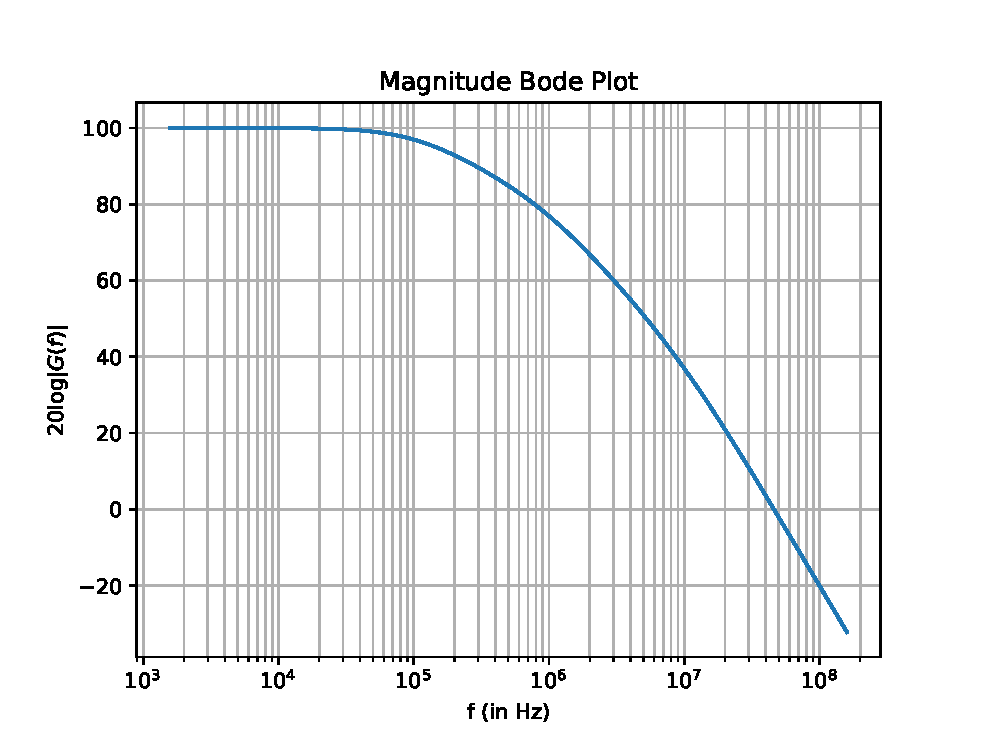
\includegraphics[width=\columnwidth]{./figs/ee18btech11014/Magnitude_Plot.eps}
	\end{center}
	\caption{Magnitude Bode Plot}
	\label{fig:Magnitude Plot}
\end{figure}

Phase Plot is \ref{fig:Phase Plot}
\begin{figure}[ht!]
	\begin{center}
		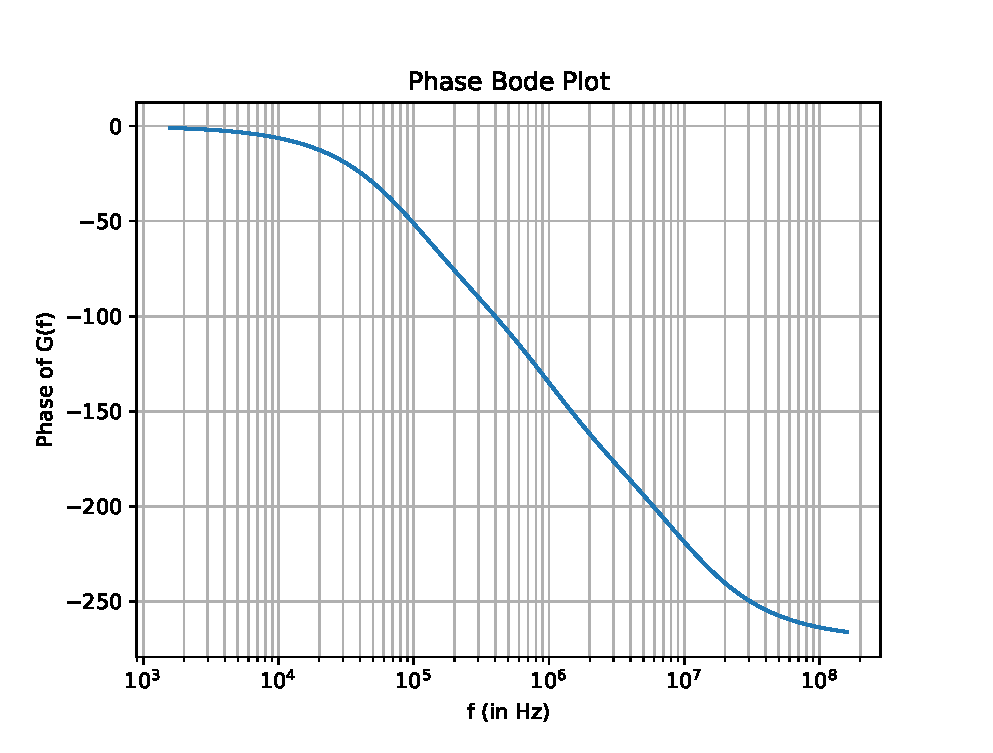
\includegraphics[width=\columnwidth]{./figs/ee18btech11014/Phase_Plot.eps}
	\end{center}
	\caption{Phase Bode Plot}
	\label{fig:Phase Plot}
\end{figure}

Python Code for Magnitude and Phase Bode Plots is at
\begin{lstlisting}
codes/ee18btech11014/Bode_Plot.py
\end{lstlisting}

%-------------------------------------------------------------------------------------------------%
%2.1.13
\item  Design a Closed-Loop Transfer Function by combining both the Open-Loop and Feedback Circuits. Also draw its Equivalent Circuit\\
\solution\\
The Closed-Loop Circuit is
\begin{figure}[ht!]
	\begin{center}
		\resizebox{\columnwidth}{!}{\begin{circuitikz}[american]

\draw (2,2)  node[op amp] (OA) {};
\draw (OA.up) -- ++(0, 0.3) node[vcc]{$+10V$};
\draw (OA.down) -- ++(0,-0.3) node[vee]{$-10V$};
\draw (OA.+) -- (0,1.5) to[vsourcesin, l= $v_{s}$] (0,0) node[ground](GND){};
\draw (OA.-) -- (0,2.5) to[R=$10\ohm$] (-2,2.5) node[ground, rotate=270](GND){};
\draw (OA.out) -- (3,2) node[label={below:$v_{a}$}]{};
\draw (3,2) to[R=$10^{2}\ohm$] (5.5,2) node[label={above:$v_{b}$}]{} to[C,l_=$\frac{10^{-9}}{2\pi}F$] (5.5,0) node[ground](GND){};
\draw (5.5,2) to[R=$10^{3}\ohm$] (8,2) node[label={above:$v_{c}$}]{} to[C,l_=$\frac{10^{-9}}{2\pi}F$] (8,0) node[ground](GND){};
\draw (8,2) to[R=$10^{4}\ohm$] (10.5,2) to[C,l_=$\frac{10^{-9}}{2\pi}F$] (10.5,0) node[ground](GND){};
\draw (10.5,2) -- (11.5,2) node[label={above:$v_{o}$}]{};
\draw (10.5,2) -- (10.5,4) to[R=$1.778\times 10^{5}\ohm$] (0,4) -- (0,2.5);

\end{circuitikz}
}
	\end{center}
	\caption{}
	\label{fig:ee18btech11014_Closed-Loop Circuit}
\end{figure}

The Equivalent Circuit of Closed-Loop Circuit is
\begin{figure}[ht!]
	\begin{center}
		\resizebox{\columnwidth}{!}{\begin{circuitikz}[american]-1
\draw (-3,0) node[ground](GND){} to[vsourcesin, l= $v_{s}$] (-3,2) to[short,-o] (0.25,2) node[label={below:$+$}]{};
\draw (0,0.1) to[R=$10\ohm$,v=$v_{f}$] (-2,0.1) node[ground](GND){}; 
\draw (0,0.1) -- (1,0.1) -- (1,4) to[R=$1.778\times 10^{5}\ohm$] (10.5,4) -- (10.5,2);


\draw (0.25,0.1) to[short,-o] (0.25,0.1) node[label={above:$-$}]{};
\draw (0.25,0.625) node[label={$v_{i}$}] {};


\draw (3,2) node[label={above:$v_{a}$}]{};
\draw (3,0) node[ground](GND){} to[vsourcesin, l= $10^5 v_{i}$] (3,2);
\draw (3,2) to[R=$10^{2}\ohm$] (5.5,2) node[label={above:$v_{b}$}]{} to[C,l_=$\frac{10^{-9}}{2\pi}F$] (5.5,0) node[ground](GND){};
\draw (5.5,2) to[R=$10^{3}\ohm$] (8,2) node[label={above:$v_{c}$}]{} to[C,l_=$\frac{10^{-9}}{2\pi}F$] (8,0) node[ground](GND){};
\draw (8,2) to[R=$10^{4}\ohm$] (10.5,2) to[C,l_=$\frac{10^{-9}}{2\pi}F$] (10.5,0) node[ground](GND){};
\draw (10.5,2) -- (11.5,2) node[label={above:$v_{o}$}]{};

\end{circuitikz}
}
	\end{center},
	\caption{}
	\label{fig:ee18btech11014_Closed-Loop Equivalent Circuit}
\end{figure}

From the Equivalent Circuit Diagram,
\begin{align}
G = \frac{v_{o}}{v_{i}} = \dfrac{10^5}{\left(1+j\frac{f}{10^{5}}\right)\left(1+j\frac{f}{10^{6}}\right)\left(1+j\frac{f}{10^{7}}\right)}\\
H = \frac{v_{f}}{v_{o}} = 5.623 \times 10^{-5}
\end{align}

The Closed-Loop Gain,
\begin{align}
v_{i} = v_{s} - v_{f}\\
\frac{v_{o}}{G} = v_{s} - Hv_{o}\\
\frac{v_{o}}{v_{s}} = \frac{G}{1+GH}
\end{align}

So, the Closed-Loop Gain,
\begin{align}
T = \frac{v_{o}}{v_{s}} = \dfrac{10^5}{5.623 + \left(1+j\frac{f}{10^{5}}\right)\left(1+j\frac{f}{10^{6}}\right)\left(1+j\frac{f}{10^{7}}\right)}
\end{align}

\end{enumerate}

\section{Assignment}
%\begin{enumerate}[label=\arabic*.,ref=\theenumi]
\begin{enumerate}[label=\thesection.\arabic*.,ref=\thesection.\theenumi]
\numberwithin{equation}{enumi}
%-------------------------------------------------------------------------------------------------%
%2.1.6
\item Find the frequency for which $PM = 90 \degree$.  Assume $H$ to be constant.
\\
%\solution Letting 
%\item Find the frequencies for which phase margins are $90\degree$ and $45\degree$ respectively?\\
\solution $\because \phase{H\brak{f}} = 1$, 
\begin{align}
\phase{G\brak{f_{90}}H\brak{f_{90}}} &= \phase{G\brak{f_{90}}} = 90\degree - 180\degree
\\
&= -90\degree
\label{eq:ee18btech11014_Gpm90}
%\\
%\implies \abs{G\brak{f_{90}}H\brak{f_{90}}} &=1
\end{align}
%
%From \eqref{eq:ee18btech11014_G_ang},
%%
%\begin{multline}
%\phi\brak{f} =
%\\
%-\sbrak{\tan ^{-1}\brak{\frac{f}{10^{5}}}+\tan ^{-1}\brak{\frac{f}{10^{6}}}+\tan ^{-1}\brak{\frac{f}{10^{7}}}}
%\end{multline}
The Bode plot in Fig. 	\ref{fig:ee18btech11014_Bode} shows that 
\begin{align}
\abs{G(f)} < 1, \quad f > 10^8
\end{align}
%
Also, 
\begin{align}
\tan^{-1}\brak{\frac{f}{10^{7}}} \approx 0, \quad f < 10^8
\end{align}

Thus, from  \eqref{eq:ee18btech11014_G_ang} and \eqref{eq:ee18btech11014_Gpm90},
%
\begin{align}
\phi\brak{f} &\approx
-\sbrak{\tan ^{-1}\brak{\frac{f}{10^{5}}}+\tan ^{-1}\brak{\frac{f}{10^{6}}}}
\\
&= -90 \degree
\\
\implies f_{90} &= 3.162 \times 10^{5}
\end{align}
after simplification.
%-------------------------------------------------------------------------------------------------%
\item Find $H$ when the $PM = 90 \degree$.
\\
\solution By definition of the PM, 
\begin{align}
\abs{G\brak{f_{90}}H\brak{f_{90}}} &=1
\\
\implies \abs{H\brak{f_{90}}} &=\frac{1}{\abs{G\brak{f_{90}}}}
\label{eq:ee18btech11014_GH_PM_90}
\end{align}
%
From \eqref{eq:ee18btech11014_G_piece},
\begin{align}
20 \log \abs{G(f)} &= 200 - 20\log(3.162 \times 10^{5})\\
&= 90 dB \\
\implies \abs{G(f)} &= 3.1625 \times 10^{4}
\\
\implies H &= 3.162 \times 10^{-5}
\end{align}
using \eqref{eq:ee18btech11014_GH_PM_90}.
%-------------------------------------------------------------------------------------------------%
\item Design the closed loop circuit for $PM = 90 \degree$
\\
\solution See Fig. 	\ref{fig:ee18btech11014_Closed-Loop Circuit alpha=90}, where Fig. 	\ref{fig:ee18btech11014_Feedback Circuit} is used for the feedback $H$ with $R_M = 0.3162 M \ohm$ and 	$R_F = 10 \ohm$.

\begin{figure}[ht!]
	\begin{center}
		\resizebox{\columnwidth}{!}{\begin{circuitikz}[american]

\draw (2,2)  node[op amp] (OA) {};
\draw (OA.up) -- ++(0, 0.3) node[vcc]{$+10V$};
\draw (OA.down) -- ++(0,-0.3) node[vee]{$-10V$};
\draw (OA.+) -- (0,1.5) to[vsourcesin, l= $v_{s}$] (0,0) node[ground](GND){};
\draw (OA.-) -- (0,2.5) to[R=$10\ohm$] (-2,2.5) node[ground, rotate=270](GND){};
\draw (OA.out) -- (3,2) node[label={below:$v_{a}$}]{};
\draw (3,2) to[R=$10^{2}\ohm$] (5.5,2) node[label={above:$v_{b}$}]{} to[C,l_=$\frac{10^{-9}}{2\pi}F$] (5.5,0) node[ground](GND){};
\draw (5.5,2) to[R=$10^{3}\ohm$] (8,2) node[label={above:$v_{c}$}]{} to[C,l_=$\frac{10^{-9}}{2\pi}F$] (8,0) node[ground](GND){};
\draw (8,2) to[R=$10^{4}\ohm$] (10.5,2) to[C,l_=$\frac{10^{-9}}{2\pi}F$] (10.5,0) node[ground](GND){};
\draw (10.5,2) -- (11.5,2) node[label={above:$v_{o}$}]{};
\draw (10.5,2) -- (10.5,4) to[R=$3.162\times 10^{5}\ohm$] (0,4) -- (0,2.5);

\end{circuitikz}
}
	\end{center}
	\caption{}
	\label{fig:ee18btech11014_Closed-Loop Circuit alpha=90}
\end{figure}

%-------------------------------------------------------------------------------------------------%
\item Repeat all the above for $PM = 45\degree$.
%-------------------------------------------------------------------------------------------------%

%-\tan^{-1}\left(f/10^{5}\right)-\tan^{-1}\left(f/10^{6}\right) = -90\\
%\tan^{-1}\left(f/10^{5}\right)+\tan^{-1}\left(f/10^{6}\right) = 90\\
%\tan^{-1}\left(f/10^{5}\right) = 90-\tan^{-1}\left(f/10^{6}\right)\\
%\tan^{-1}\left(f/10^{5}\right) = \cot^{-1}\left(f/10^{6}\right)\\
%\tan^{-1}\left(f/10^{5}\right) = \tan^{-1}\left(10^{6}/f\right)\\
%f^{2} = 10^{11}\\
%f = 3.162 \times 10^{5}
%\end{align}
%
%So, the approximate value of $f$ at which Phase Margin is $90\degree$ is $f=3.162 \times 10^{5} Hz$.\\

%Similarly let Phase Margin be $\alpha = 45\degree$. Then,
%\begin{align}
%\alpha = \phi - (-180\degree)\\
%\phi = -180\degree + \alpha\\
%\phi = -135\degree
%\end{align}
%
%So, by the definition of Phase-Margin, at $\phi = -135\degree$ , $|GH| = 1 $.  The value of $\phi = -135\degree$ aproximately at poles $f=10^{6} Hz$. 
%
%So, the approximate value of $f$ at which Phase Margin is $45\degree$ is $f=10^{6}$.\\
%%-------------------------------------------------------------------------------------------------%
%%2.1.7
%\item Find the minimum values of Closed-Loop Voltage Gain for which phase margins are $90\degree$ and  $45\degree$ respectively\\
%\solution\\
%For $\alpha=90\degree$,
%\begin{align}
%f=3.162 \times 10^{5}
%\end{align}
%By substituting $f$ in Open-Loop Gain $G(f)$ (assuming poles are far part), 
%\begin{align}
%G(f) = 200 - 20log(3.162 \times 10^{5})\\
%G(f) = 90 dB \\
%G = 3.1625 \times 10^{4}
%\end{align}
%
%At that $f=3.162 \times 10^{5}$, 
%\begin{align}
%H = \frac{1}{G}\\
%H = 3.162 \times 10^{-5}
%\end{align}
%
%The minimum value of Closed-Loop Gain occurs at $|GH| \gg 1$ and the value of Closed-Loop Gain is $T=\frac{1}{H}$
%
%\begin{align}
%T = \frac{1}{H} = 3.1625 \times 10^{4}
%\end{align}
%
%\textbf{So, The minimum value of Closed-Loop Gain with Phase Margin equal to $\alpha=90\degree$ is $T_{min} = 3.1625 \times 10^{4}$.}\\
%
%For $\alpha=45\degree$,
%\begin{align}
%f=10^{6}
%\end{align}
%By substituting $f$ in Open-Loop Gain $G(f)$ (assuming poles are far part), 
%\begin{align}
%G(f) = 200 - 20log(10^{6})\\
%G(f) = 80 dB \\
%G = 10^{4}
%\end{align}
%
%At that $f = 10^{6}$, 
%\begin{align}
%H = \frac{1}{G}\\
%H = 10^{-4}
%\end{align}
%
%The minimum value of Closed-Loop Gain occurs at $|GH| \gg 1$ and the value of Closed-Loop Gain is $T=\frac{1}{H}$
%
%\begin{align}
%T = \frac{1}{H} = 10^{4}
%\end{align}
%
%\textbf{So, The minimum value of Closed-Loop Gain with Phase Margin equal to $\alpha=45\degree$ is $T_{min} = 10^{4}$.}\\
%%-------------------------------------------------------------------------------------------------%
%
%\item Design a Feedback circuit for Phase Margin $\alpha=45^{\circ}$.\\
%\solution
%\begin{figure}[ht!]
%	\begin{center}
%		\resizebox{\columnwidth/2}{!}{\begin{circuitikz}[american]
\ctikzset{tripoles/mos style/arrows}
\draw (1,2) to[short, -o] (0,2) node[label={below:$v_{o}$}]{};
\draw (1,2) to[R=$100k\ohm$] (2,2) -- (3,2) to[R=$10\ohm$] (3,0) node[ground](GND){};
\draw (3,2) to[short, -o] (4,2) node[label={below:$v_{f}$}]{};
\end{circuitikz}
}
%	\end{center},
%	\caption{}
%	\label{fig:ee18btech11014_alpha=45}
%\end{figure}
%\begin{align}
%v_{f} = \frac{10}{10 + 10^{5}} \times v_{o}\\
%v_{f} \approx 10^{-4} v_{o}\\
%\frac{v_{f}}{v_{o}} \approx 10^{-4}\\
%H(s) = 10^{-4}
%\end{align}
%%-------------------------------------------------------------------------------------------------%
%
%\item Design a Feedback circuit for Phase Margin $\alpha=90^{\circ}$.\\
%\solution
%\begin{figure}[ht!]
%	\begin{center}
%		\resizebox{\columnwidth/2}{!}{\begin{circuitikz}[american]
\ctikzset{tripoles/mos style/arrows}
\draw (1,2) to[short, -o] (0,2) node[label={below:$v_{o}$}]{};
\draw (1,2) to[R=$0.3162 M\ohm$] (2,2) -- (3,2) to[R=$10\ohm$] (3,0) node[ground](GND){};
\draw (3,2) to[short, -o] (4,2) node[label={below:$v_{f}$}]{};
\end{circuitikz}
}
%	\end{center},
%	\caption{}
%	\label{fig:ee18btech11014_alpha=90}
%\end{figure}
%\begin{align}
%v_{f} = \frac{10}{10 + 3.162\times 10^{5}} \times v_{o}\\
%v_{f} \approx 3.162\times 10^{-5} v_{o}\\
%\frac{v_{f}}{v_{o}} \approx 3.162\times 10^{-5}\\
%H(s) = 3.162\times 10^{-5}
%\end{align}
%%-------------------------------------------------------------------------------------------------%
%
%\item  Design a Closed-Loop Transfer Function by combining both the Open-Loop and Feedback Circuits for phase Margin $\alpha=45^{\circ}$. Also draw its Equivalent Circuit\\
%\solution\\
%The Closed-Loop Circuit is
%\begin{figure}[ht!]
%	\begin{center}
%		\resizebox{\columnwidth}{!}{\begin{circuitikz}[american]

\draw (2,2)  node[op amp] (OA) {};
\draw (OA.up) -- ++(0, 0.3) node[vcc]{$+10V$};
\draw (OA.down) -- ++(0,-0.3) node[vee]{$-10V$};
\draw (OA.+) -- (0,1.5) to[vsourcesin, l= $v_{s}$] (0,0) node[ground](GND){};
\draw (OA.-) -- (0,2.5) to[R=$10\ohm$] (-2,2.5) node[ground, rotate=270](GND){};
\draw (OA.out) -- (3,2) node[label={below:$v_{a}$}]{};
\draw (3,2) to[R=$10^{2}\ohm$] (5.5,2) node[label={above:$v_{b}$}]{} to[C,l_=$\frac{10^{-9}}{2\pi}F$] (5.5,0) node[ground](GND){};
\draw (5.5,2) to[R=$10^{3}\ohm$] (8,2) node[label={above:$v_{c}$}]{} to[C,l_=$\frac{10^{-9}}{2\pi}F$] (8,0) node[ground](GND){};
\draw (8,2) to[R=$10^{4}\ohm$] (10.5,2) to[C,l_=$\frac{10^{-9}}{2\pi}F$] (10.5,0) node[ground](GND){};
\draw (10.5,2) -- (11.5,2) node[label={above:$v_{o}$}]{};
\draw (10.5,2) -- (10.5,4) to[R=$10^{5}\ohm$] (0,4) -- (0,2.5);

\end{circuitikz}
}
%	\end{center}
%	\caption{}
%	\label{fig:ee18btech11014_Closed-Loop Circuit alpha=45}
%\end{figure}
%
%The Equivalent Circuit of Closed-Loop Circuit is
%\begin{figure}[ht!]
%	\begin{center}
%		\resizebox{\columnwidth}{!}{\begin{circuitikz}[american]-1
\draw (-3,0) node[ground](GND){} to[vsourcesin, l= $v_{s}$] (-3,2) to[short,-o] (0.25,2) node[label={below:$+$}]{};
\draw (0,0.1) to[R=$10\ohm$,v=$v_{f}$] (-2,0.1) node[ground](GND){}; 
\draw (0,0.1) -- (1,0.1) -- (1,4) to[R=$10^{5}\ohm$] (10.5,4) -- (10.5,2);


\draw (0.25,0.1) to[short,-o] (0.25,0.1) node[label={above:$-$}]{};
\draw (0.25,0.625) node[label={$v_{i}$}] {};


\draw (3,2) node[label={above:$v_{a}$}]{};
\draw (3,0) node[ground](GND){} to[vsourcesin, l= $10^5 v_{i}$] (3,2);
\draw (3,2) to[R=$10^{2}\ohm$] (5.5,2) node[label={above:$v_{b}$}]{} to[C,l_=$\frac{10^{-9}}{2\pi}F$] (5.5,0) node[ground](GND){};
\draw (5.5,2) to[R=$10^{3}\ohm$] (8,2) node[label={above:$v_{c}$}]{} to[C,l_=$\frac{10^{-9}}{2\pi}F$] (8,0) node[ground](GND){};
\draw (8,2) to[R=$10^{4}\ohm$] (10.5,2) to[C,l_=$\frac{10^{-9}}{2\pi}F$] (10.5,0) node[ground](GND){};
\draw (10.5,2) -- (11.5,2) node[label={above:$v_{o}$}]{};

\end{circuitikz}
}
%	\end{center},
%	\caption{}
%	\label{fig:ee18btech11014_Closed-Loop Equivalent Circuit alpha=45}
%\end{figure}
%
%From the Equivalent Circuit Diagram,
%\begin{align}
%G(s) = \dfrac{10^5}{\left(1+\frac{s}{2\pi 10^{5}}\right)\left(1+\frac{s}{2\pi 10^{6}}\right)\left(1+\frac{s}{2\pi 10^{7}}\right)}\\
%H(s) = \frac{v_{f}}{v_{o}} = 10^{-4}
%\end{align}
%
%The Closed-Loop Gain,
%\begin{align}
%v_{i} = v_{s} - v_{f}\\
%\frac{v_{o}}{G} = v_{s} - Hv_{o}\\
%\frac{v_{o}}{v_{s}} = \frac{G}{1+GH}
%\end{align}
%
%So, the Closed-Loop Gain,
%\begin{align}
%T(s) = \frac{v_{o}}{v_{s}} = \dfrac{10^5}{10 + \left(1+s\frac{s}{2\pi 10^{5}}\right)\left(1+\frac{s}{2\pi 10^{6}}\right)\left(1+j\frac{s}{2\pi 10^{7}}\right)}
%\end{align}
%%-------------------------------------------------------------------------------------------------%
%
%\item  Design a Closed-Loop Transfer Function by combining both the Open-Loop and Feedback Circuits for phase Margin $\alpha=90^{\circ}$. Also draw its Equivalent Circuit\\
%\solution\\
%The Closed-Loop Circuit is
%\begin{figure}[ht!]
%	\begin{center}
%		\resizebox{\columnwidth}{!}{\begin{circuitikz}[american]

\draw (2,2)  node[op amp] (OA) {};
\draw (OA.up) -- ++(0, 0.3) node[vcc]{$+10V$};
\draw (OA.down) -- ++(0,-0.3) node[vee]{$-10V$};
\draw (OA.+) -- (0,1.5) to[vsourcesin, l= $v_{s}$] (0,0) node[ground](GND){};
\draw (OA.-) -- (0,2.5) to[R=$10\ohm$] (-2,2.5) node[ground, rotate=270](GND){};
\draw (OA.out) -- (3,2) node[label={below:$v_{a}$}]{};
\draw (3,2) to[R=$10^{2}\ohm$] (5.5,2) node[label={above:$v_{b}$}]{} to[C,l_=$\frac{10^{-9}}{2\pi}F$] (5.5,0) node[ground](GND){};
\draw (5.5,2) to[R=$10^{3}\ohm$] (8,2) node[label={above:$v_{c}$}]{} to[C,l_=$\frac{10^{-9}}{2\pi}F$] (8,0) node[ground](GND){};
\draw (8,2) to[R=$10^{4}\ohm$] (10.5,2) to[C,l_=$\frac{10^{-9}}{2\pi}F$] (10.5,0) node[ground](GND){};
\draw (10.5,2) -- (11.5,2) node[label={above:$v_{o}$}]{};
\draw (10.5,2) -- (10.5,4) to[R=$3.162\times 10^{5}\ohm$] (0,4) -- (0,2.5);

\end{circuitikz}
}
%	\end{center}
%	\caption{}
%	\label{fig:ee18btech11014_Closed-Loop Circuit alpha=90}
%\end{figure}
%
%The Equivalent Circuit of Closed-Loop Circuit is
%\begin{figure}[ht!]
%	\begin{center}
%		\resizebox{\columnwidth}{!}{\begin{circuitikz}[american]-1
\draw (-3,0) node[ground](GND){} to[vsourcesin, l= $v_{s}$] (-3,2) to[short,-o] (0.25,2) node[label={below:$+$}]{};
\draw (0,0.1) to[R=$10\ohm$,v=$v_{f}$] (-2,0.1) node[ground](GND){}; 
\draw (0,0.1) -- (1,0.1) -- (1,4) to[R=$3.162\times 10^{5}\ohm$] (10.5,4) -- (10.5,2);


\draw (0.25,0.1) to[short,-o] (0.25,0.1) node[label={above:$-$}]{};
\draw (0.25,0.625) node[label={$v_{i}$}] {};


\draw (3,2) node[label={above:$v_{a}$}]{};
\draw (3,0) node[ground](GND){} to[vsourcesin, l= $10^5 v_{i}$] (3,2);
\draw (3,2) to[R=$10^{2}\ohm$] (5.5,2) node[label={above:$v_{b}$}]{} to[C,l_=$\frac{10^{-9}}{2\pi}F$] (5.5,0) node[ground](GND){};
\draw (5.5,2) to[R=$10^{3}\ohm$] (8,2) node[label={above:$v_{c}$}]{} to[C,l_=$\frac{10^{-9}}{2\pi}F$] (8,0) node[ground](GND){};
\draw (8,2) to[R=$10^{4}\ohm$] (10.5,2) to[C,l_=$\frac{10^{-9}}{2\pi}F$] (10.5,0) node[ground](GND){};
\draw (10.5,2) -- (11.5,2) node[label={above:$v_{o}$}]{};

\end{circuitikz}
}
%	\end{center},
%	\caption{}
%	\label{fig:ee18btech11014_Closed-Loop Equivalent Circuit alpha=90}
%\end{figure}
%
%From the Equivalent Circuit Diagram,
%\begin{align}
%G(s) = \dfrac{10^5}{\left(1+\frac{s}{2\pi 10^{5}}\right)\left(1+\frac{s}{2\pi 10^{6}}\right)\left(1+\frac{s}{2\pi 10^{7}}\right)}\\
%H(s) = \frac{v_{f}}{v_{o}} = 3.162\times 10^{-5}
%\end{align}
%
%The Closed-Loop Gain,
%\begin{align}
%v_{i} = v_{s} - v_{f}\\
%\frac{v_{o}}{G} = v_{s} - Hv_{o}\\
%\frac{v_{o}}{v_{s}} = \frac{G}{1+GH}
%\end{align}
%
%So, the Closed-Loop Gain,
%\begin{align}
%T(s) = \frac{v_{o}}{v_{s}} = \dfrac{10^5}{3.162 + \left(1+s\frac{s}{2\pi 10^{5}}\right)\left(1+\frac{s}{2\pi 10^{6}}\right)\left(1+j\frac{s}{2\pi 10^{7}}\right)}
%\end{align}
\end{enumerate}

\end{document}
